\subsection{Modelling relevant aspects in EA}
\visHeader

The first step is to get the existing metamodel into EA. A complete and automatic import of existing Ecore files in EA is currently not possible and therefore,
\emph{relevant parts} of the existing metamodel (\texttt{GenModel}) have to be modelled manually in EA. Although this might sound frightening (especially for
large, complex metamodels), the emphasis here on \emph{relevant} indicates that only elements that are used for the transformation have to be present in EA and
can be added iteratively as the transformation grows.

\begin{enumerate}

\item[$\blacktriangleright$] To specify our example transformation, open Eclipse and create a new metamodel project named \texttt{EcoreToGenModel}, and select
the \texttt{Add Demo Specification} option in the project wizard window. 

\item[$\blacktriangleright$] You can either delete or ignore the \texttt{DemoTestSuite} project raising errors, and switch to EA by double-clicking the created
\texttt{Ecore\-To\-Gen\-Model.eap} file.

\item[$\blacktriangleright$] Explore the project browswer and make of note of the packages already present in EA under \texttt{eMoflon Languages}, especially
\texttt{Ecore} which we shall use for this transformation.

\item[$\blacktriangleright$] Create a new package named \texttt{GenModel} in \texttt{eMoflon Languages}, and add a new Ecore diagram. Model the elements as
depicted in Fig.~\ref{fig_gMM}. You'll need to create the three EClasses on the left, but \texttt{Ecore::EPackage} and \texttt{Ecore::EClass} can be
drag-and-dropped, pasted as links from the project browser. 

\newpage

\begin{figure}[htbp]
\begin{center}  
	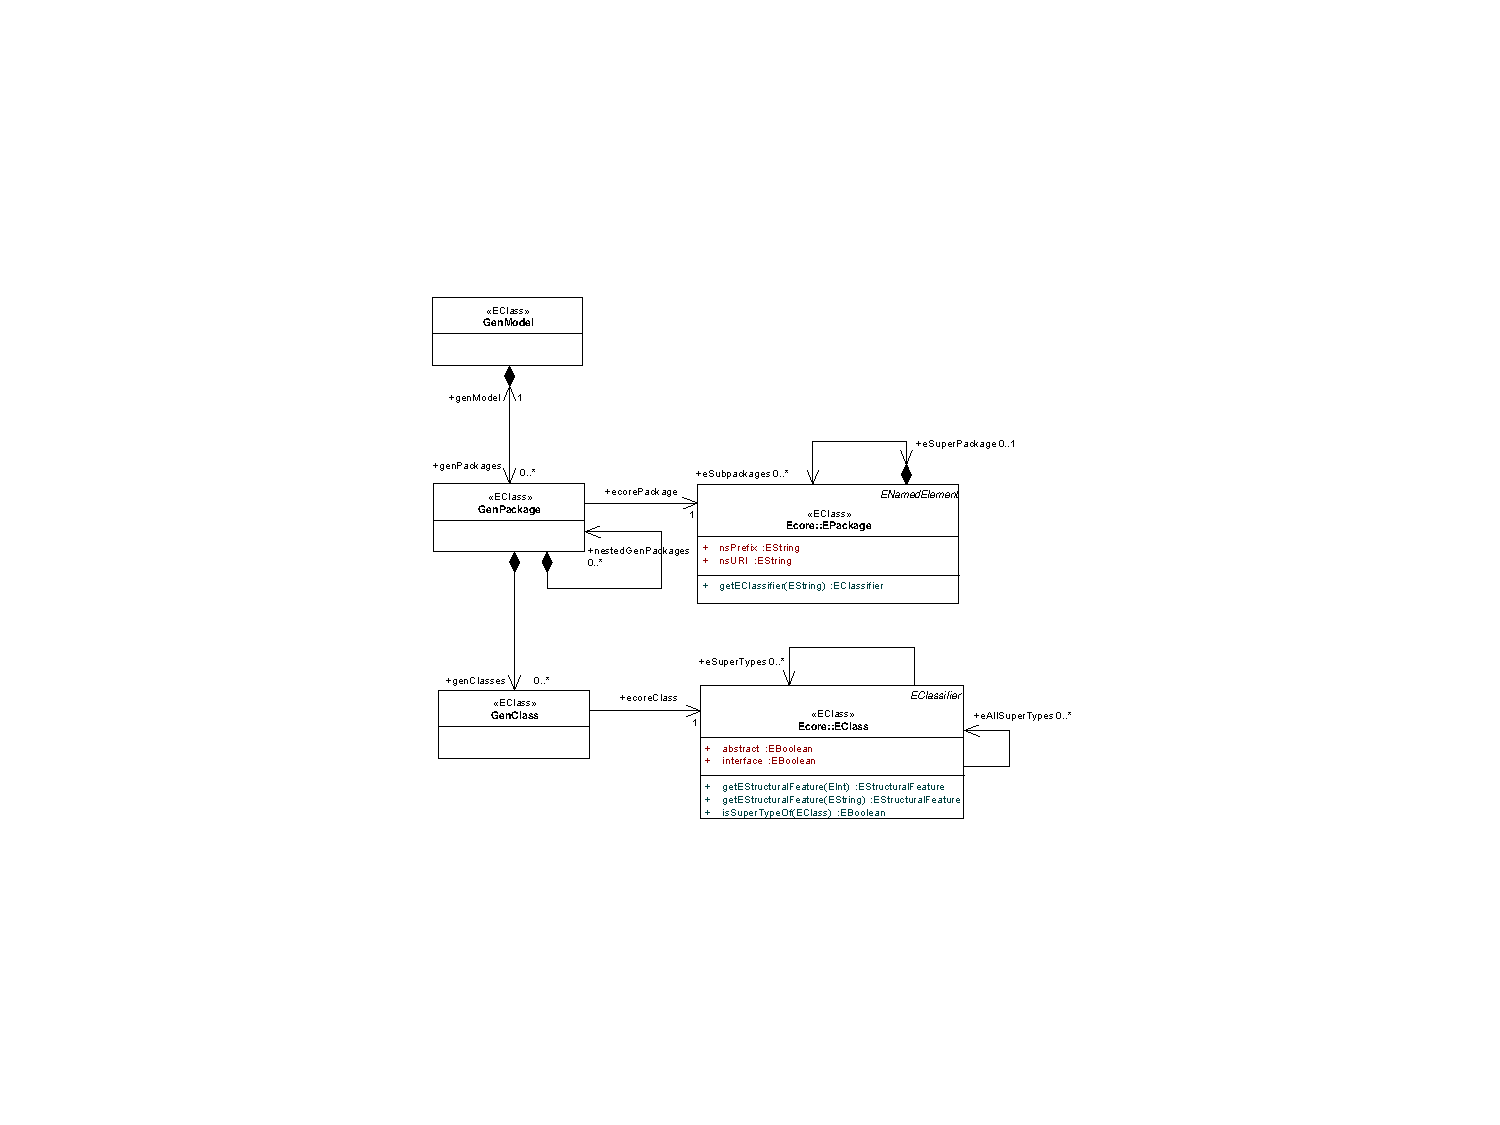
\includegraphics[width=1.0\textwidth]{CDGenmodel.pdf}
	\caption{Metamodel of \texttt{GenModel}}  
\label{fig_gMM}
\end{center}
\end{figure} 

\item[$\blacktriangleright$] Please note that the actual \texttt{GenModel} metamodel contains lots more elements, but this subset is sufficient for our task.

\item[$\blacktriangleright$] Create another \texttt{Ecore2GenModel} package and digram to contain the \texttt{Transformer} class with the methods as depicted in
Fig.~\ref{fig_e2gm}.

\item[$\blacktriangleright$] Implement their SDMs as depicted in Figs.~\ref{fig_pack2gm} and \ref{fig_transf}.
\end{enumerate}

\begin{figure}[htbp]
\begin{center}  
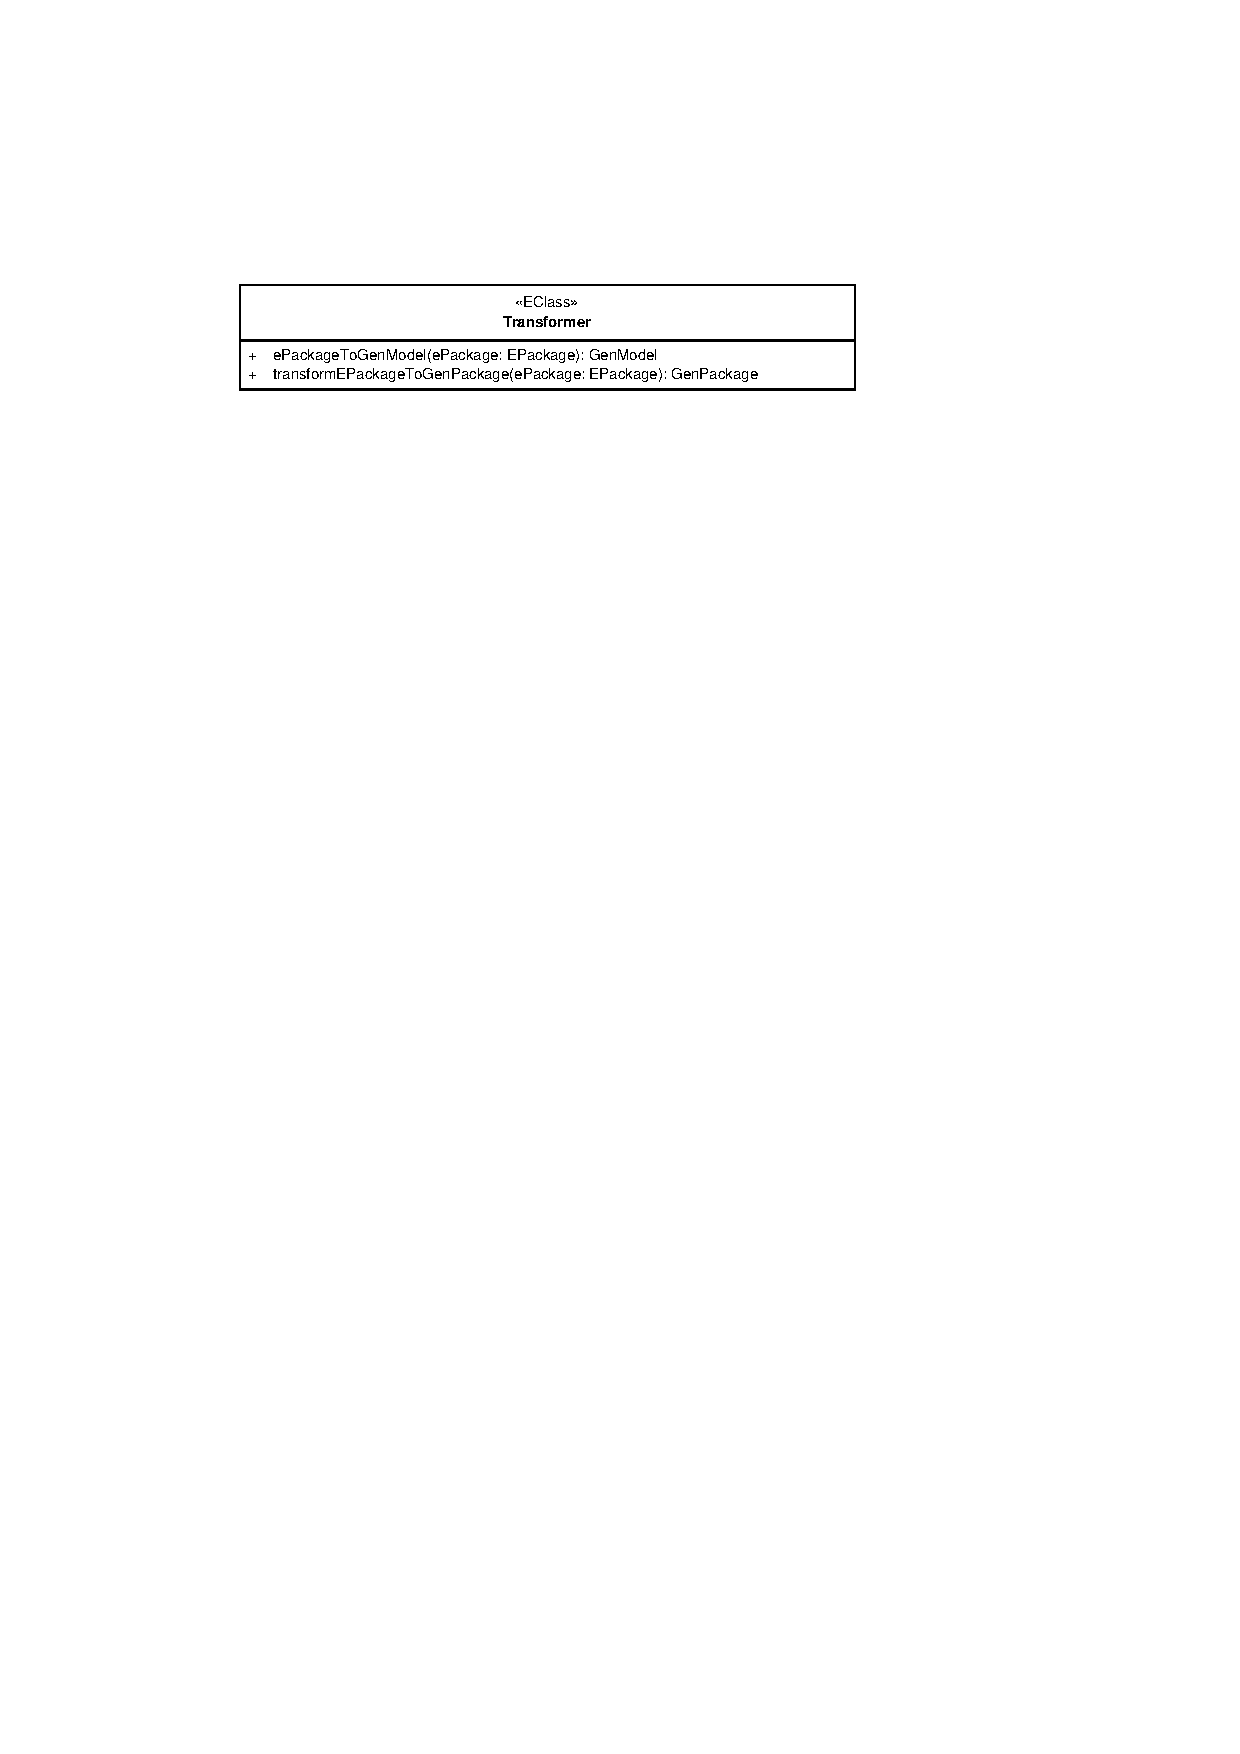
\includegraphics[width=0.8\textwidth]{CDTransformer.pdf}
\caption{Methods in \texttt{Transformer}}  
\label{fig_e2gm}
\end{center}
\end{figure} 

\begin{figure}[htbp]
\begin{center}  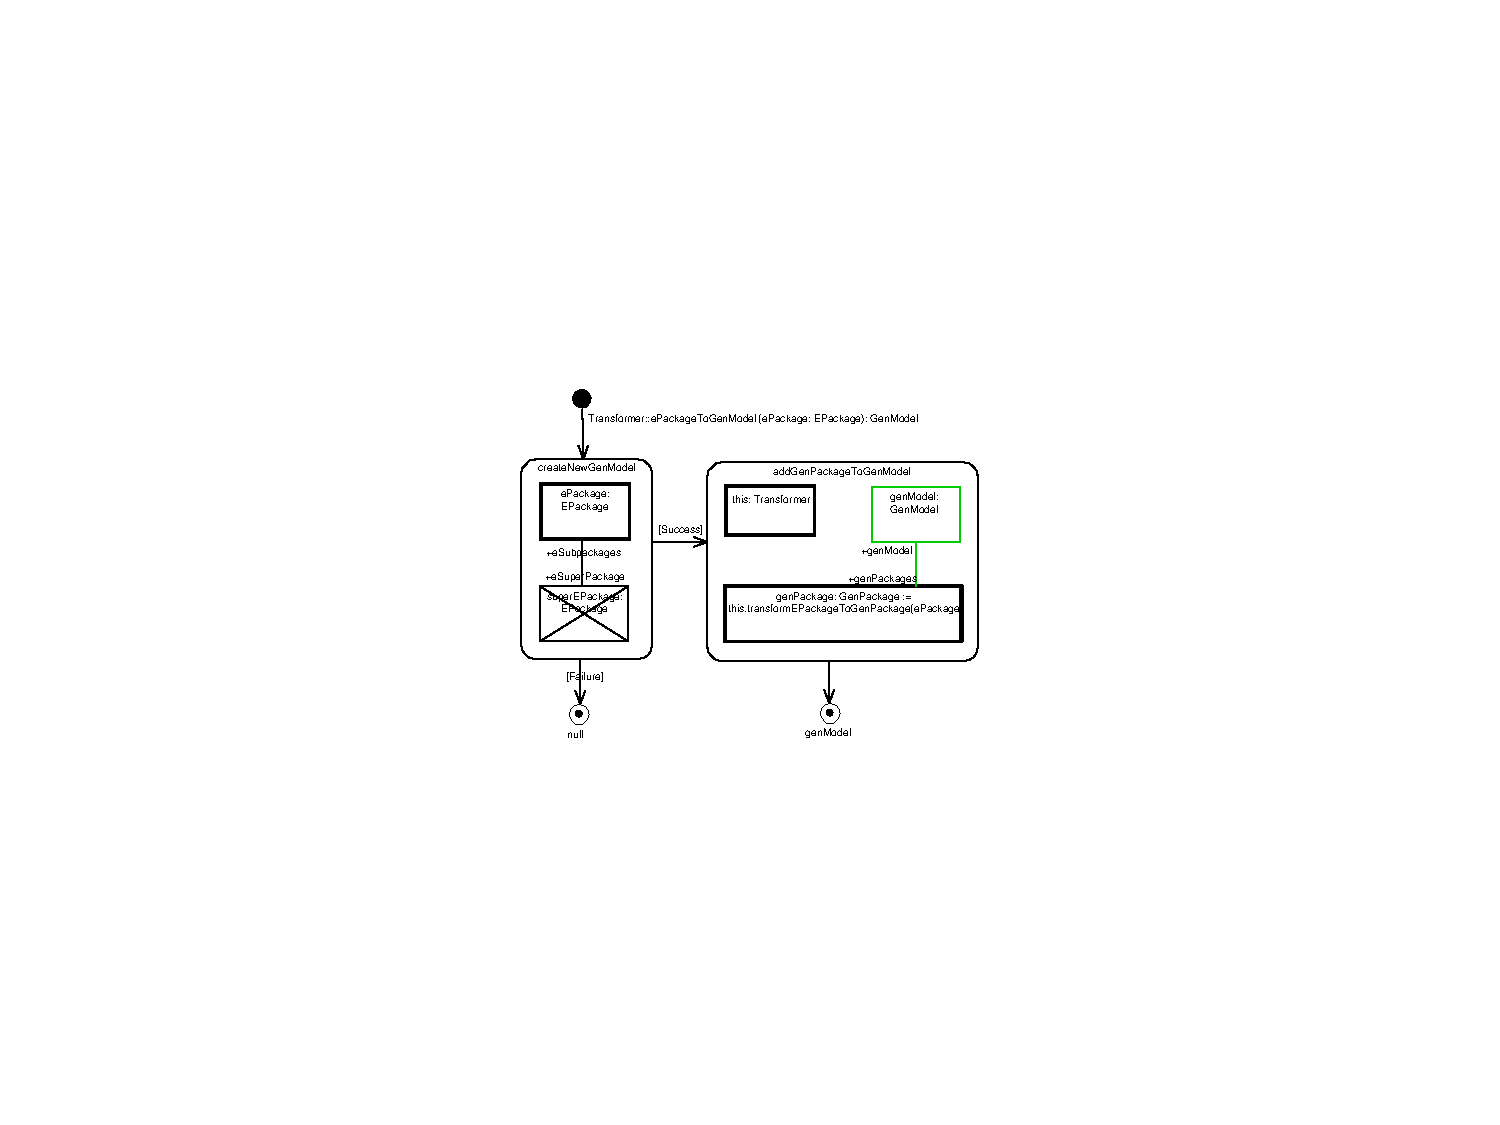
\includegraphics[width=0.8\textwidth]{SDMePackageToGenModel.pdf}
        \caption{Main method for \texttt{EPackage} to \texttt{GenModel} transformation}  
  \label{fig_pack2gm}
\end{center}
\end{figure} 

\begin{figure}[htbp]
\begin{center}  
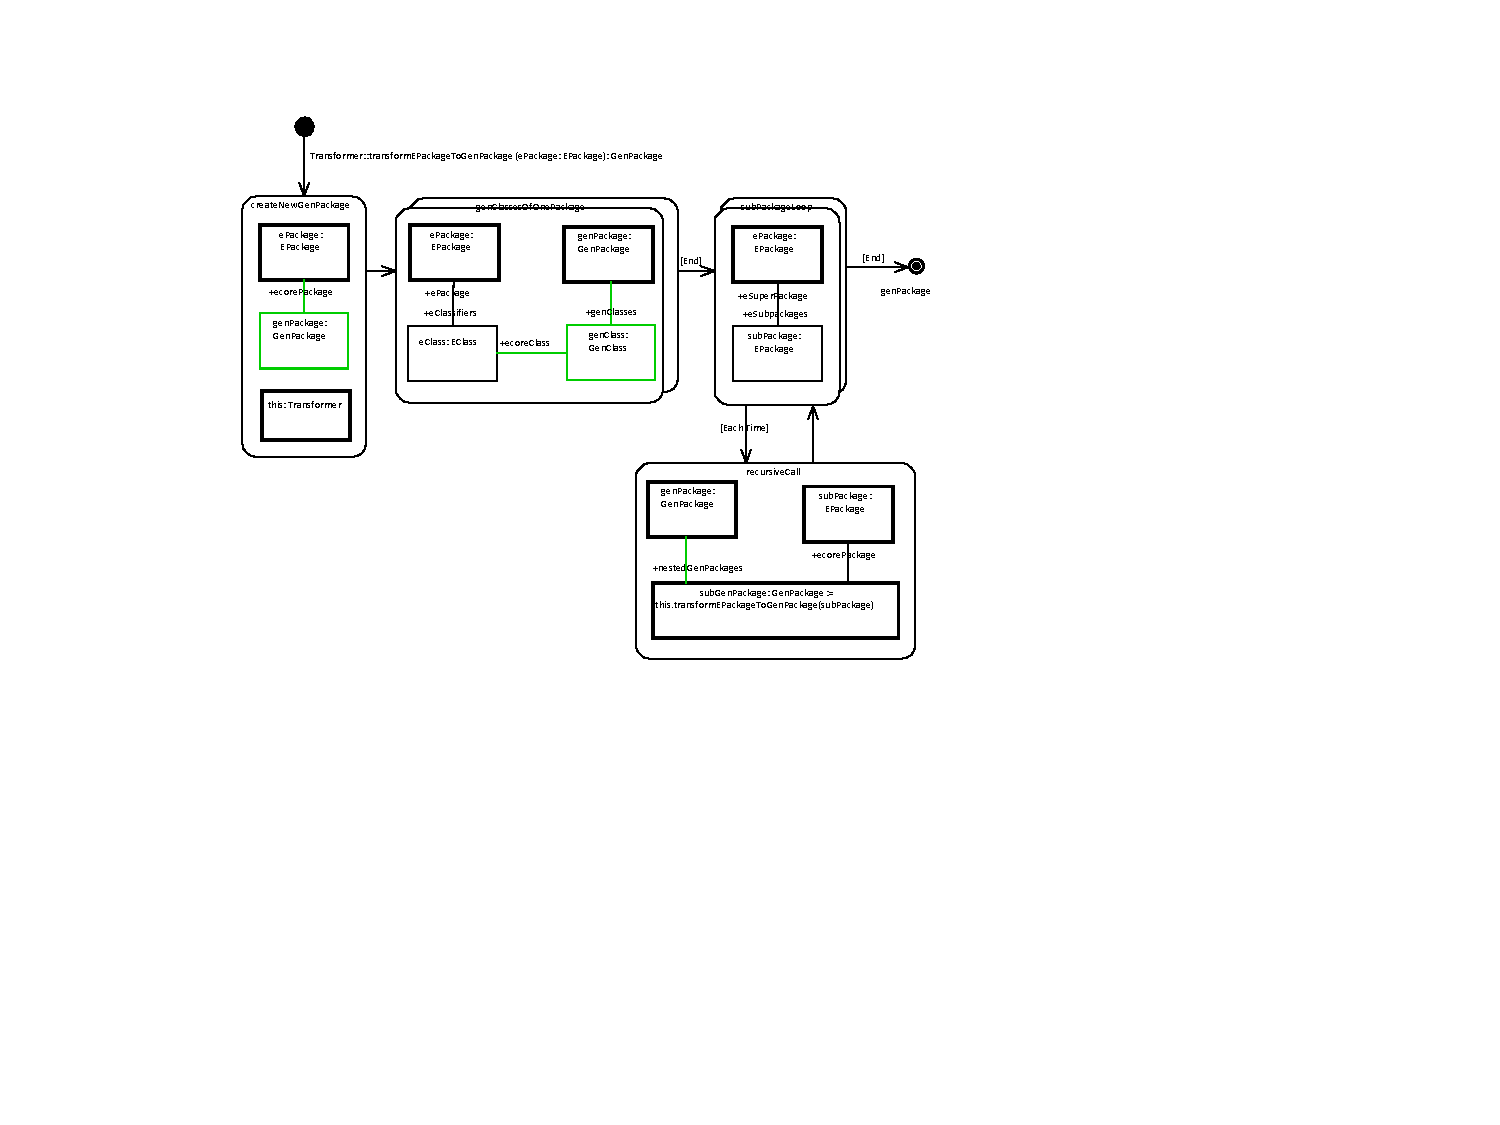
\includegraphics[width=1.0\textwidth]{SDMtransformEpackageToGenPackage.pdf}
\caption{Helper function to transform all \texttt{EPackages} to \texttt{GenPackages}}  
\label{fig_transf}
\end{center}
\end{figure} 

